\documentclass[a4paper]{article}
\usepackage{fullpage}
\usepackage[scaled]{helvet}
\usepackage{graphicx}
\usepackage{tabularx}
%\usepackage{floatflt}
\usepackage{lastpage}

\usepackage{fancyhdr}

% Fix \paragraph to have a newline
\makeatletter
\renewcommand\paragraph{\@startsection{paragraph}{4}{\z@}%
  {-3.25ex\@plus -1ex \@minus -.2ex}%
  {1.5ex \@plus .2ex}%
  {\normalfont\normalsize\bfseries}}
\makeatother

% Put in a background picture
\newcommand\BackgroundPic{
\put(0,0){
\parbox[b][\paperheight]{\paperwidth}{%
\vfill
\centering
\includegraphics[width=\paperwidth,keepaspectratio]{background_top.pdf}%
%\vfill
%\includegraphics[width=\paperwidth,keepaspectratio]{background_bottom.pdf}%
\vfill
}}}

\setcounter{secnumdepth}{4}	% Number \paragraphs

\renewcommand\maketitle{
%\ifpdf
\pdfinfo{
   /Author (\getauthor)
   /Title  (\getprojectname  - \gettitle)
   /Producer (John Hodge)
}
%\fi


\begin{titlepage}

\begin{center}

\vspace{1cm}

\textsc{\LARGE \getprojectname}\\[0.5cm]
\textsc{\huge \gettitle}\\[0.5cm]
\rule{0.9\textwidth}{0.7pt} \\[0.75cm]
% Authors
\emph{\getauthor} \\[0.5cm]
% Client
Client: \emph{\getclient} \\[0.5cm]

CITS3200 Professional Computing 2011 \\
University of Western Australia Crawley, WA, 6009

\vspace{2cm}
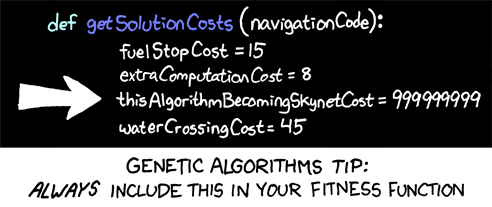
\includegraphics{../534-genetic_algorithms.png} \\
\centering{\footnotesize XKCD \#534 - Genetic Algorithms - CC BY-NC 2.5}

\end{center}

\end{titlepage}
}

\def\csharp{\ensuremath{C\sharp } }

\def\getprojectname{}
\def\projectname#1{\gdef\getprojectname{#1}}
\def\getclient{}
\def\client#1{\gdef\getclient{#1}}
\makeatletter
\newcommand\gettitle{\@title}
\newcommand\getauthor{\@author}
\makeatother

\renewcommand*\familydefault{\sfdefault}{\normalsize}	% Sets the font
